%
		\section{Plasma-Wall Interaction}\label{sec:sheathphysics}
%
%       !!! DIESER GANZE ABSCHNITT GEHÖRT IN DEN TEIL VORHER INTEGRIERT, 
%           SO DASS MAN DA DIE SCHICHT WIRKLICH VERSTEHEN KANN !!!
%           LOGIK:1) SCHICHT 2) CCRF-EFFEKTE
%
            In contrast to the plasma bulk, the charge densities do not satisfy the quasi-neutrality condition in a distance of $d$ from the wall. Because of the negative potential around a wall the transport processes of electrons and ions are perturbed. The potential barrier reflects electrons of low kinetic energies, although both particle species diffuse into the sheath. Because continuity has to be satisfied, e.g\@ $j\ix{e}=j\ix{i}$ at the sheath-boundary, negative space charges build up and the corresponding electric fields accelerate the ions to match this condition.\\
            The physicals law which characterise those transport processes are derived in the following sections. 
%
			\subsection{Child-Langmuir Law}\label{sec:langmuirlaw}
%			
				\begin{wrapfigure}[18]{r}{0.5\textwidth}
					\centering%
					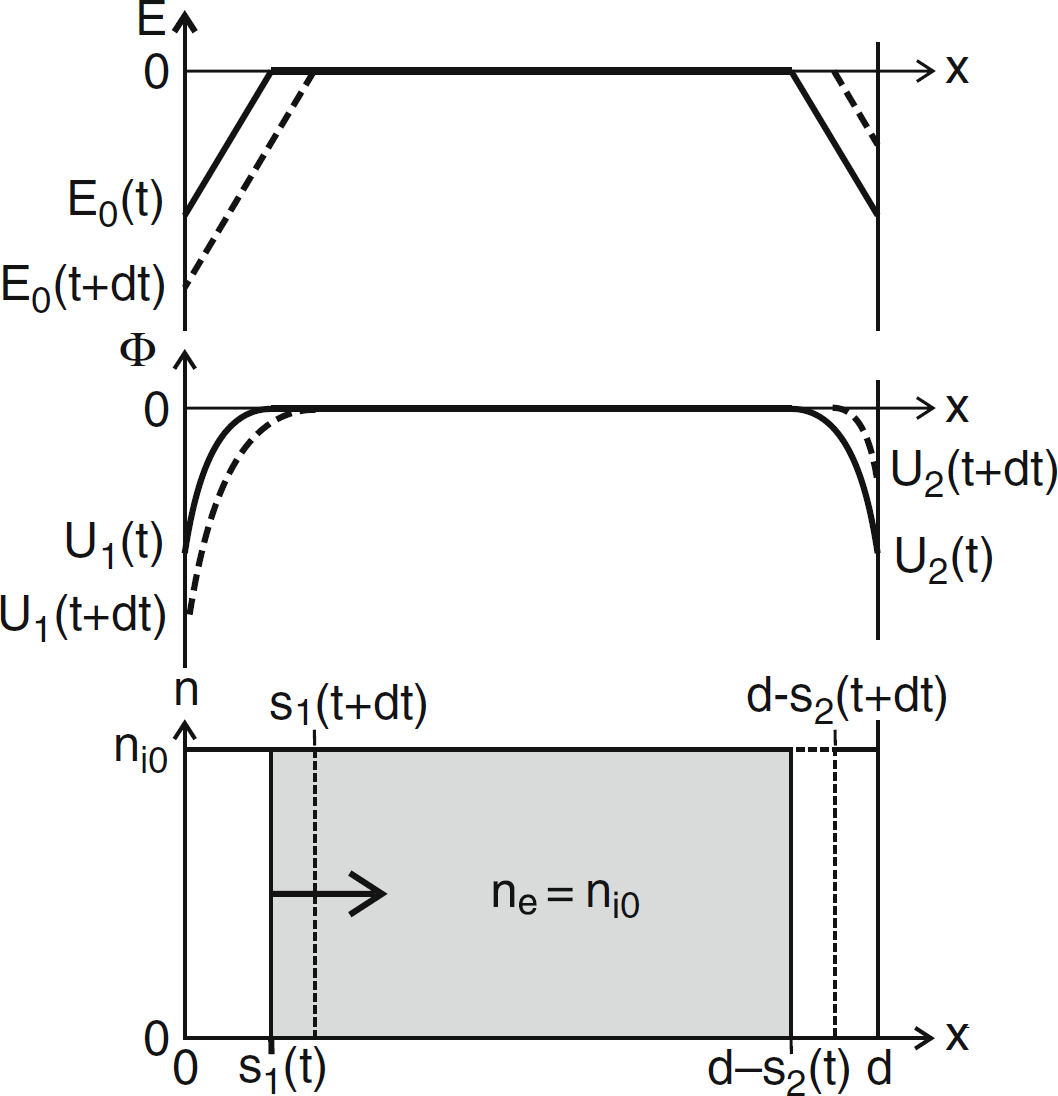
\includegraphics[width=0.45\textwidth]{figures/displacement_current_piel.png}%
					\caption{%
						One dimensional density, potential and electric field for an asymmetric, harmonically %
						driven discharge.~\cite{Piel10}}\label{fig:displacementcurrent}
				\end{wrapfigure}
%
			In an one-dimensional model, a negatively charged wall at $x=0$ creates a potential barrier for electrons of thermal velocity, e.g.\@ $|\Phi(0)-\Phi(d)|\ll k\ix{B}T\ix{e}/e\,$. The thickness of the space-charge sheath here is $d$ and the sheath-boundary therefore at $x=-d$ (see~\autoref{fig:sheath_piel}). It is usually the size of a few Debye-length $\lambda\ix{D}$. The electron density $n\ix{e}(x)$ towards the wall can be written with a \emph{Boltzmann} distribution function $f\ix{B}(\Phi)\sim\exp(e\Delta\Phi/k\ix{B}T\ix{e})\,$~\cite{Piel10}. This means that the electron density decreases exponentially towards the negatively charged wall.\\
			It can be assumed that the sheath thickness $d\ll s\ix{mfp,i}$ the mean free path of the ions inside the plasma bulk. Hence the ions enter the pre-sheath collisionless at a speed $v\ix{i,0}$. The ion and electron densities are therefore:
%
				\begin{align}
					n\ix{i}(x)=n\ix{i}(d&){\left(1-\frac{2e\Phi(x)}%
						{m\ix{i}v\ix{i,0}^{2}}\right)}^{-1/2}%
%						\nonumber\\[0.2cm]%
						\quad\text{~and~}\quad
						n\ix{e}=n\ix{e}(d)\exp&\left(%
						\frac{e(\Phi(x)-\Phi(d))}{k\ix{B}T\ix{e}}\right)\,%
						\label{equ:ionandelectrondens}
				\end{align}
%
			At the boundary between bulk and pre-sheath, the walls potential vanishes because of the plasmas shielding capabilities. Furthermore, one can assume that the kinetic energy of the ions at this point is smaller than the potential energy for the acceleration inside the pre-sheath, e.g.\@ $m\ix{i}v\ix{i,0}^{2}\ll |e\Phi(x)|$. Using \emph{Poisson's} equation gives an expression for the potential $\Phi(x)$ Solving this, and using the unperturbed ion current $j\ix{i}=n\ix{i}(d)ev\ix{i,0}$, one yields the result by \emph{Langmuir} in~\autoref{equ:langmuirpot}:
%
				\begin{align}
					\Delta\Phi\cong-\frac{en\ix{i}{\left(-d\right)}%
						}{\varepsilon\ix{0}}{\left(-\frac{2e\Phi{%
						\left(x\right)}}{m\ix{i}v\ix{i,0}^2}\right)}^{-\frac{1}{2}}%
					\quad\Rightarrow\quad%
					\Phi{\left(x\right)}=&{\left({\left(\frac{3}{4}{\left(x+d%
						\right)}\right)}^4{\left(\frac{j\ix{i}}{\varepsilon\ix{0}%
						}\right)}^2\frac{m\ix{i}}{2e}\right)}^{\frac{1}{3}}%
						\label{equ:langmuirpot}
				\end{align}
%
				Solving again for $j\ix{i}$ yields the \emph{Child-Langmuir Law} (see~\autoref{equ:childlangmuirlaw}). This equation defines the ion current as a function of the unperturbed plasma bulk. In other words, the sheath changes its thickness in dependency of the discharge parameters, always satisfying the ion current defined by the Child-Langmuir Law:
%
				\begin{align}
					j\ix{i}=\frac{4}{9}&\varepsilon\ix{0}{\left(\frac{2e{%
						\left(\Phi{\left(-d\right)}-\Phi{\left(0\right)}%
						\right)}^3}{m\ix{i}d^2}\right)}^{\frac{1}{2}}%
				    	\label{equ:childlangmuirlaw}
				\end{align}
%				
				The \emph{Child-Langmuir Law} yields an expression for the relation between potential and current on a wall in a space-charge limited plasma region, e.g\@ the sheath. It characterises transport processes between a floating wall and the plasma bulk. Therefore it is important to understand, for example the oscillation of the sheath boundary in rf plasmas or secondary emission processes at walls.